\SourcePage{287}{290}
\section{Symmetry under permutations}

For a system consisting of only two particles, we could assert that its coordinate wave functions for stationary states, $\varphi(\mathbf r_1,\mathbf r_2)$, must be either symmetric or antisymmetric. For a system containing an arbitrary number of particles, however, the solutions of the Schrödinger equation (the coordinate wave functions) need not be symmetric or antisymmetric under interchange of every pair of particles, unlike the complete wave functions, which include a spin factor. The reason is that interchanging only the coordinates of two particles does not yet amount to physically interchanging the particles themselves. Here the physical identity of the particles implies only that the system's Hamiltonian is invariant under particle permutations. Consequently, if one function solves the Schrödinger equation, then the functions obtained from it by the various permutations of its variables are solutions as well.

We first give some general remarks about permutations. A system of $N$ particles admits $N!$ distinct permutations. Imagine that all particles have been numbered; every permutation can then be represented by a particular ordering of the numbers $1,2,3,\ldots$ Any such ordering can be produced from the natural ordering $1,2,3,\ldots$ by successively interchanging pairs of particles. A permutation is called \emph{even} or \emph{odd} according as it is effected by an even or odd number of pairwise interchanges. Let $\widehat P$ denote the permutation operators for the $N$ particles, and introduce $\delta_P$, equal to $+1$ when $\widehat P$ is an even permutation and to $-1$ when it is odd. If $\varphi$ is symmetric in all the particles, then
\[
 \widehat P\varphi=\varphi,
\]

\SourcePage{288}{291}
whereas, if the function is antisymmetric in all the particles,
\[
 \widehat P\varphi=\delta_P\varphi.
\]

From an arbitrary function $\varphi(\mathbf r_1,\mathbf r_2,\ldots,\mathbf r_N)$ one can form a symmetric function by the operation of \emph{symmetrization}, written as
\begin{equation}
 \varphi_{\mathrm{sym}}=\operatorname{const}\cdot\sum_P\widehat P\varphi,
 \tag{63.1}
\end{equation}
where the sum extends over every possible permutation. The construction of an antisymmetric function (an operation also called \emph{alternation}) can be written
\begin{equation}
 \varphi_{\mathrm{asym}}=\operatorname{const}\cdot\sum_P\delta_P\widehat P\varphi.
 \tag{63.2}
\end{equation}

We return to the behavior of the wave functions $\varphi$ of a system of identical particles under permutations\footnote{In mathematical terms, the problem is to find the irreducible representations of the permutation group. Detailed accounts of the mathematical theory of permutation groups may be found in: H.~Weyl, \emph{Group Theory and Quantum Mechanics}; M.~Hamermesh, \emph{Group Theory and Applications to Problems in Physics}; I.~G.~Kaplan, \emph{Symmetry in Many-Electron Systems}.}. Mathematically, the symmetry of the system's Hamiltonian $\widehat H$ in all particles means that it commutes with every permutation operator $\widehat P$. These operators, however, do not commute with one another and hence cannot all be reduced simultaneously to diagonal form. Thus the wave functions $\varphi$ cannot be chosen so that each is symmetric or antisymmetric under every separate pairwise interchange\footnote{Only a two-particle system has just one permutation operator, which can be reduced to diagonal form simultaneously with the Hamiltonian.}.

Our task is to determine the possible symmetry types, under permutations of the variables, of functions $\varphi(\mathbf r_1,\mathbf r_2,\ldots,\mathbf r_N)$ of $N$ variables (or of sets of several such functions).

The symmetry must be incapable of further increase: every additional symmetrization or alternation applied to these functions must turn them either into linear combinations of the same functions or identically into zero.

\SourcePage{289}{292}
We already know two operations that produce functions of maximal symmetry: symmetrization in all variables and alternation in all variables. They can be generalized as follows.

Partition the complete set of $N$ variables $\mathbf r_1,\mathbf r_2,\ldots,\mathbf r_N$ (or, equivalently, the indices $1,2,3,\ldots,N$) into several rows containing $N_1,N_2,\ldots$ elements (variables), where $N_1+N_2+\ldots=N$. Such a partition can be displayed pictorially by a diagram (a \emph{Young diagram}) in which each of the numbers $N_1,N_2,\ldots$ is represented by a row of cells. Figure~21, for example, shows the partitions $6+4+4+3+3+1+1$ and $7+5+5+3+1+1$ for $N=22$; one of the numbers $1,2,3,\ldots$ is to be placed in every square. If the rows are arranged in decreasing order of length (as in Fig.~21), the diagram consists not only of successive horizontal rows but also of vertical columns.

\begin{figure}[ht]
\centering
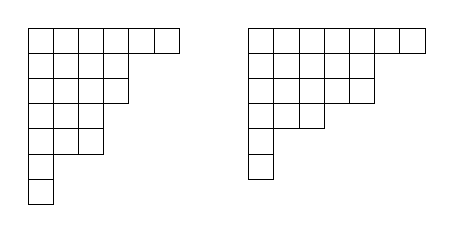
\begin{tikzpicture}[x=3.2mm,y=3.2mm,line width=.35pt]
 \foreach \r/\n in {0/6,1/4,2/4,3/3,4/3,5/1,6/1}{\foreach \c in {0,...,\numexpr\n-1\relax}{\draw (\c,-\r) rectangle ++(1,-1);}}
 \begin{scope}[xshift=28mm]
 \foreach \r/\n in {0/7,1/5,2/5,3/3,4/1,5/1}{\foreach \c in {0,...,\numexpr\n-1\relax}{\draw (\c,-\r) rectangle ++(1,-1);}}
 \end{scope}
\end{tikzpicture}
\par\smallskip {\small Fig. 21}
\end{figure}

Symmetrize an arbitrary function $\varphi(\mathbf r_1,\mathbf r_2,\ldots,\mathbf r_N)$ in the variables belonging to each row. Alternation may thereafter be performed only on variables from different rows; alternation in a pair of variables lying in the same row plainly gives zero identically.

Choose one variable from every row. Without loss of generality these variables may be regarded as occupying the first cells of their rows, since after symmetrization their ordering among the cells of a row is immaterial; now alternate in the chosen variables. Next strike out the first column and alternate in variables chosen one from each row of the shortened diagram; they may again be regarded as occupying the first cells of the shortened rows. Continuing in this manner, we obtain a function first symmetrized in the variables of every row and then alternated in those of every column. After alternation, of course, the function generally ceases to be symmetric in the variables of each row; symmetry remains only for variables in the cells of the first row that project beyond the other rows.

Assign the $N$ variables in different ways to the rows of the Young diagram (their placement among the cells of any one row

\SourcePage{290}{293}
is immaterial). This procedure gives a collection of functions that are carried into one another by an arbitrary permutation of the variables\footnote{The order of symmetrization and alternation could instead be reversed: first alternate over the variables in each column, and then symmetrize over those in the rows. This produces nothing new, however, because the functions obtained by the two procedures are linear combinations of one another.}. It must nevertheless be stressed that these functions are not all linearly independent. In general, the number of independent functions is smaller than the number of possible assignments of the variables to the rows of the diagram; we shall not examine this point further here\footnote{A set of independent functions carried into one another forms a basis for an irreducible representation of the permutation group. The number of these functions is the dimension of the representation. For particles of spin $1/2$, it is found in Problem~1 of this section.}.


Thus every Young diagram specifies a particular symmetry type of functions under permutations. By constructing every Young diagram possible for a given $N$, we obtain all possible symmetry types. This reduces to partitioning the number $N$ in every possible way into a sum of smaller terms, with $N$ itself included among the allowed partitions. For $N=4$, for example, the partitions are $4$, $3+1$, $2+2$, $2+1+1$, and $1+1+1+1$.

A Young diagram can be associated with each energy level of the system; it specifies the permutation symmetry of the corresponding solutions of the Schrödinger equation. In general, a given energy value corresponds to several distinct functions that transform into one another under permutations. This ``permutation degeneracy'' is connected with the already noted noncommutativity of the operators $\widehat P$, each of which commutes with the Hamiltonian (cf. §~10, p.~48). It does not, however, signify any additional physical degeneracy of the energy levels. Multiplied by spin functions, all these distinct coordinate wave functions enter one particular combination---the complete wave function---which satisfies the condition of symmetry or antisymmetry according to the particles' spin.

For any given $N$, the various symmetry types always include two that are each represented by a single function. In one case the function is symmetric in every variable, and in the other it is antisymmetric (the Young diagram in the former case

\SourcePage{291}{294}
is a single row of $N$ boxes, while in the latter it is a single column).


We now pass to the spin wave functions $\chi(\sigma_1,\sigma_2,\ldots,\sigma_N)$. Their symmetry types under particle permutations are described by the same Young diagrams, with the particle spin projections playing the role of variables. The question arises: which diagram must correspond to the spin function when the diagram of the coordinate function is given? Suppose first that the particles have integral spin. The complete wave function $\psi$ must then be symmetric in all particles. This requires the spin and coordinate functions to have symmetry described by the same Young diagram, while $\psi$ is expressed as a particular bilinear combination of the two sets of functions. We shall not consider the construction of this combination here.

Suppose instead that the particles have half-integral spin. The complete wave function must then be antisymmetric in all particles. It can be shown that the Young diagrams of the coordinate and spin functions must be dual: each is obtained from the other by interchanging rows and columns (the two diagrams in Fig.~21 furnish an example).

We examine more closely the important case of particles with spin $1/2$, such as electrons. Each spin variable $\sigma_1,\sigma_2,\ldots$ can assume only the two values $\pm1/2$. A function antisymmetric in any two variables vanishes when those variables have equal values. It follows that $\chi$ can be alternated only in pairs of variables: upon alternation in three variables, at least two of them necessarily have equal values, and the result is identically zero.

For a system of electrons, therefore, the Young diagrams of the spin functions can contain columns only one or two cells long (that is, no more than two rows); in the Young diagrams for the coordinate functions, the analogous restriction applies to row lengths. Consequently, the number of possible permutation-symmetry types for $N$ electrons equals the number of partitions of $N$ into ones and twos. For even $N$ it is $N/2+1$ (partitions containing $0,1,\ldots,N/2$ twos), and for odd $N$ it is $(N+1)/2$ (partitions containing $0,1,\ldots,(N-1)/2$ twos). Figure~22 shows the possible Young diagrams, both coordinate and spin, for $N=4$.

It is readily seen that each such symmetry type (each Young diagram) corresponds to a definite total spin $S$ of the electron system. We shall represent

\SourcePage{292}{295}
the spin functions in spinor form, as a spinor $\chi^{\lambda\mu\ldots}$ of rank $N$, whose indices---each associated with the spin of one particle---are the variables placed in the cells of the Young diagrams.

\begin{figure}[ht]
\centering
\begin{tikzpicture}[x=5mm,y=5mm,line width=.35pt]
 \node at (-1.1,-2) {$\varphi$}; \node at (-1.1,-5.5) {$\chi$};
 \foreach \r/\n in {0/1,1/1,2/1,3/1}{\draw (0,-\r) rectangle ++(1,-1);}
 \foreach \r/\n in {0/2,1/1,2/1}{\foreach \c in {0,...,\numexpr\n-1\relax}{\draw (3+\c,-\r) rectangle ++(1,-1);}}
 \foreach \r/\n in {0/2,1/2}{\foreach \c in {0,...,\numexpr\n-1\relax}{\draw (7.5+\c,-\r) rectangle ++(1,-1);}}
 \foreach \c in {0,...,3}{\draw (\c,-5) rectangle ++(1,-1);}
 \foreach \r/\n in {0/3,1/1}{\foreach \c in {0,...,\numexpr\n-1\relax}{\draw (6+\c,-5-\r) rectangle ++(1,-1);}}
 \foreach \r/\n in {0/2,1/2}{\foreach \c in {0,...,\numexpr\n-1\relax}{\draw (11+\c,-5-\r) rectangle ++(1,-1);}}
 \node at (2,-6.8) {$S=2$}; \node at (7.5,-7.8) {$S=1$}; \node at (12,-7.8) {$S=0$};
\end{tikzpicture}
\par\smallskip {\small Fig. 22}
\end{figure}

Consider a spin Young diagram with two rows containing $N_1$ and $N_2$ boxes, respectively ($N_1+N_2=N$, $N_1\geq N_2$). Each of the first $N_2$ columns has two boxes, so the spinor must be antisymmetric in each corresponding pair of indices. By contrast, it must be symmetric in the indices occupying the final $n=N_1-N_2$ boxes of the first row. As we know, a rank-$N$ spinor of this kind reduces to a symmetric spinor of rank $n$, and the latter has total spin $S=n/2$. In terms of the Young diagrams for the coordinate functions, therefore, a diagram having $n$ one-box rows corresponds to a state whose total spin is $S=n/2$. For even $N$, the total spin may take the integer values from 0 through $N/2$; for odd $N$, it may take the half-integer values from $1/2$ through $N/2$, as required.


This one-to-one correspondence between Young diagrams and total spin is specific to systems of spin-$1/2$ particles; for a system of only two particles, we already encountered it in the preceding section. For $N$ particles of spin $s$, the spin wave function is formed from a product of $N$ symmetric spinors of rank $2s$, and is consequently a spinor of rank $2Ns$. When this spinor is symmetrized according to a particular Young diagram with $N$ boxes, its independent components can usually be combined into several sets of linear combinations, each associated with a different value of the system's total spin $S$.


Just as the Young diagram for the spin functions of spin-$1/2$ particles cannot have columns containing more than two cells, so for particles of arbitrary spin $s$ the column length must not exceed $2s+1$ cells.

If the number of particles $N$ is an integral multiple of $2s+1$, the possible Young diagrams include a rectangular one in which every column contains $2s+1$ cells. This diagram corresponds to one definite value of the total spin, $S=0$. Hence any two spin Young diagrams that can be joined to form a rectangle

\SourcePage{293}{296}
of height $2s+1$ correspond to the same values of $S$\footnote{For example, when $s=1$, the following pairs of diagrams have this property:
\begin{center}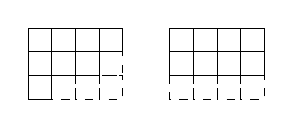
\begin{tikzpicture}[x=3mm,y=3mm,line width=.35pt]
\foreach \r/\n in {0/4,1/3,2/1}{\foreach \c in {0,...,\numexpr\n-1\relax}{\draw (\c,-\r) rectangle ++(1,-1);}}
\draw[dashed] (3,-1) rectangle ++(1,-1);
\foreach \c in {1,2,3}{\draw[dashed] (\c,-2) rectangle ++(1,-1);}
\foreach \r/\n in {0/4,1/4}{\foreach \c in {0,...,\numexpr\n-1\relax}{\draw (6+\c,-\r) rectangle ++(1,-1);}}
\foreach \c in {0,...,3}{\draw[dashed] (6+\c,-2) rectangle ++(1,-1);}
\end{tikzpicture}\end{center}
Complementary diagrams are drawn with solid and dashed lines.}. This conclusion is simply a consequence of the fact that, when two angular momenta are added, their resultant can vanish only if the two angular momenta have equal magnitudes.

To conclude this section, return to the circumstance noted earlier (see the note on p.~86): for systems of several identical particles, one cannot assert that the wave function of the lowest-energy stationary state has no nodes. We can now refine that observation and explain its origin.

A nodeless wave function (here we mean the coordinate function) must necessarily be symmetric in all particles. If it were antisymmetric under interchange of any pair of particles, say 1 and 2, it would vanish at $\mathbf r_1=\mathbf r_2$. Yet for a system of three or more electrons, a completely symmetric coordinate wave function is not allowed at all: the Young diagram of the coordinate function cannot contain a row longer than two cells. Thus, although the Schrödinger-equation solution belonging to the lowest eigenvalue has no nodes, as follows from the theorem of the calculus of variations, that solution may be physically inadmissible. The normal state of the system then corresponds to an eigenvalue other than the lowest one, and its wave function will in general have nodes. More generally, this situation occurs for particles of half-integral spin $s$ in systems containing more than $2s+1$ particles. In systems composed of bosons, by contrast, a completely symmetric coordinate wave function is always possible.
